\documentclass{hw-template}

\title{NE511 Homework 1}
\author{Kyle Hansen}
\date{12 February 2026}

\usepackage{cancel}

\renewcommand{\defeq}{\stackrel{\text{def}}{=}}




\begin{document}

\maketitle{}

\section{Core cycle Beta-physical}

Physical beta $\beta^{ph}$ can be found using the equation

\begin{equation}
    \beta^{ph} = \frac{\sum_i \beta_i \nu_{i, k} \sum_g \sum_j \nu \Sigma_{f, j, i, g}V_j \Phi_{j, g}}     {\sum_j \nu \Sigma_{f, j, i, g}V_j \Phi_{j, g}}.
\end{equation}

In other words, this is a sum of $\beta$ for each isotope, weighted by total neutron production rate for each isotope. 

From given reactor power, power is proportional to $\Sigma_f$, assuming each isotope has the same recoverable fission energy. Further assuming that the full reactor has uniform flux and cross sections, this sum can be expressed (for each precursor group) as

\begin{equation}
    \beta^{ph}_k = \frac{\sum_i \beta_{i,k} \Sigma_{f, i}\nu_{i}}  {\sum_i \Sigma_{f, i}\nu_{i}},
\end{equation}

and 

\begin{equation}
    \beta^{ph} = \sum_{k=1}^{6}\beta^{ph}_k.
\end{equation}

Using this formula, the total delayed neutron yield at each point in the cycle is shown in \autoref{tab:yields}.



\begin{table}
    \centering
    \caption{Delayed neutron yields}\label{tab:yields}
    \begin{tabular}{r|l|l}
        \hline
        Time & $\beta^{ph}$ & \% Change from BOC \\
        \hline\hline
        BOC  &   0.005985   &  0\\
        MOC1 &   0.005735   & $-4.36$\\
        MOC2 &   0.005489   & $-9.04$\\
        EOC  &   0.005011    & $-19.4$
    \end{tabular}
\end{table}

Using the formula $l_{dj} = l_p + \frac{1}{\lambda_j}$ and $\overline{l} = (1-\beta)l_p + \sum_j \beta_j l_{dj}$, the average neutron lifetime is 0.0789 s at BOC, and 0.0674 at EOC, a change of $-14.55$ percent.


\section{Decay Constant Data}

In the precursor balance equation,

\begin{equation}
    \frac{d c_k}{dt} = -\lambda_k c_k + \sum_{i=1}^{N} \Sigma_{fi} \phi \nu_{dki},
\end{equation}

the population of each precursor group is just sum of the population of each precursor belonging to that group, $c_k = \sum_{i \in k} c_i$, so the group decay constant is found with

\begin{equation}
    \lambda_k =\frac{ \sum_{i \in k} \lambda_i n_i  }{\sum_{i \in k}  n_i}.
\end{equation}

The decay constants are known to relatively little uncertainty, but $n_i$, which comes from fission product yields, is prohibitively difficult to measure per-isotope and comes with a very high uncertainty. 


\section{Fission fractions}

Assuming that that the energy spectrum is linear between each group boundary, the numbered values $\chi_i$ are the delayed spectrum and the un-numbered values $\chi$ are the prompt fission spectrum, the proportion of delayed neutrons that can cause fission is $0.023$, while the proportion of delayed neutrons that can cause fission is $0.655$-- the delayed neutrons are emitted at lower energies on average than prompt neutrons, and are thus less important in a fast-fission reactor.

\clearpage

\begin{figure}
    \centering
    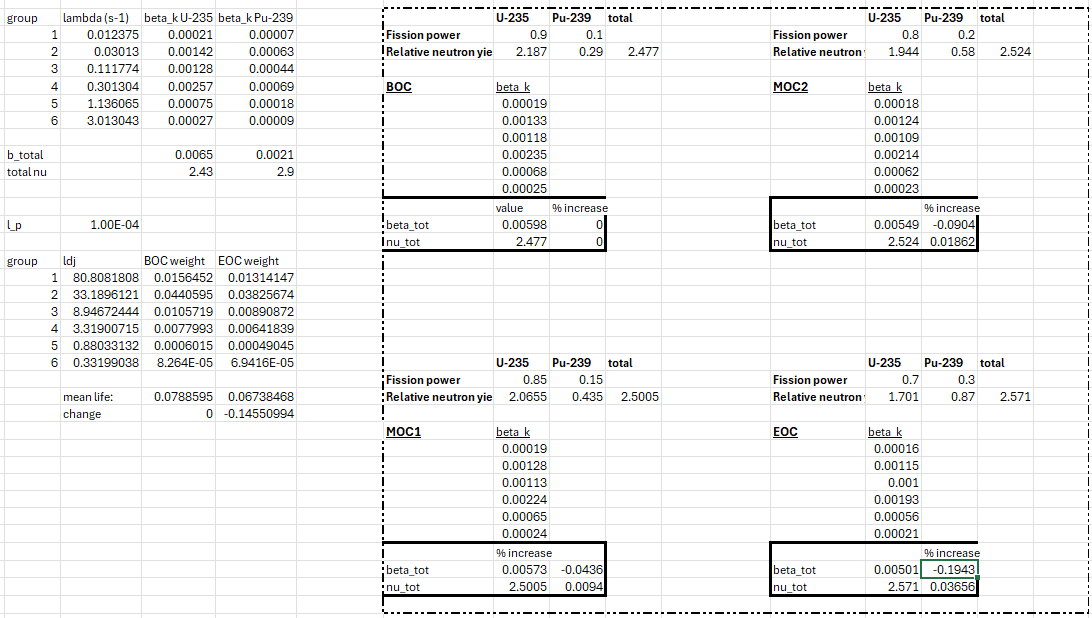
\includegraphics[width=\textwidth]{prob_1.png}
    \caption{Problem 1}
\end{figure}

\begin{figure}
    \centering
    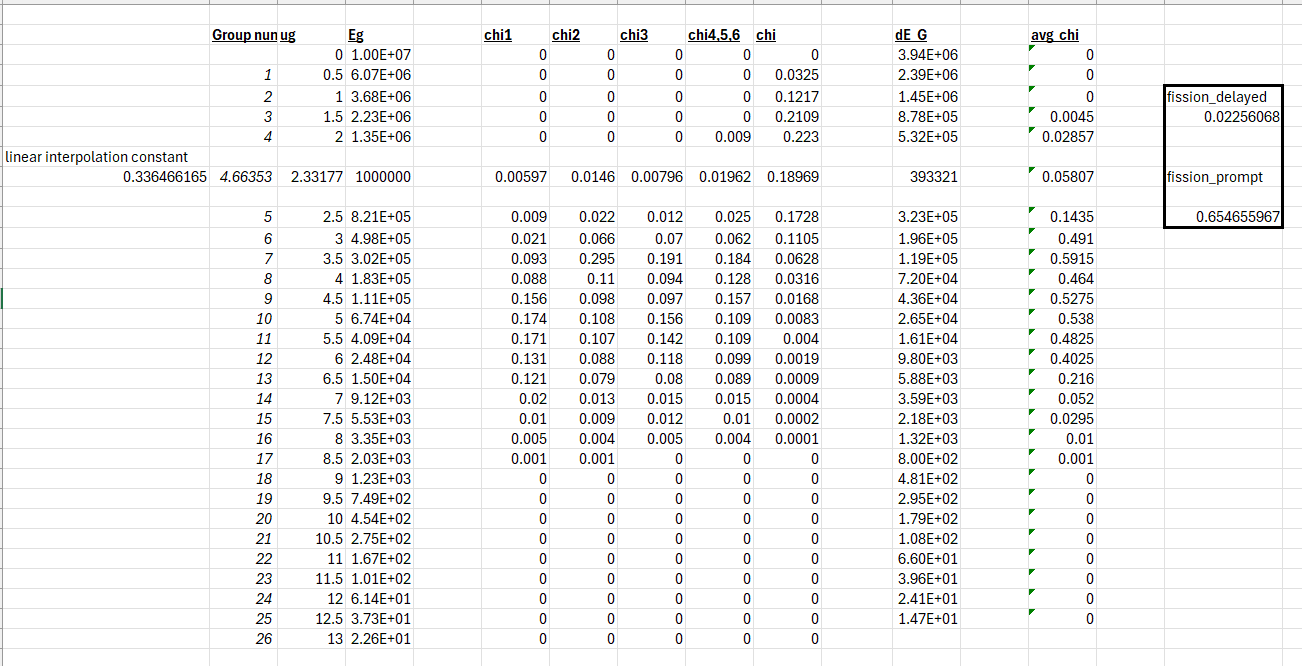
\includegraphics[width=\textwidth]{prob_3.png}
    \caption{Problem 1}
\end{figure}



\end{document}
